\documentclass[crop,tikz]{standalone}
\usetikzlibrary{%
    arrows,
    arrows.meta,
    automata,
    backgrounds,
    calc,
    decorations.pathreplacing,
    fit,
    matrix,
    positioning,
    scopes,
    shadows
}
\usepackage[linguistics]{forest}
\usepackage[charter]{mathdesign}
\tikzset{headarrow/.style = {-{Latex[length=.5em]}}}

\begin{document}
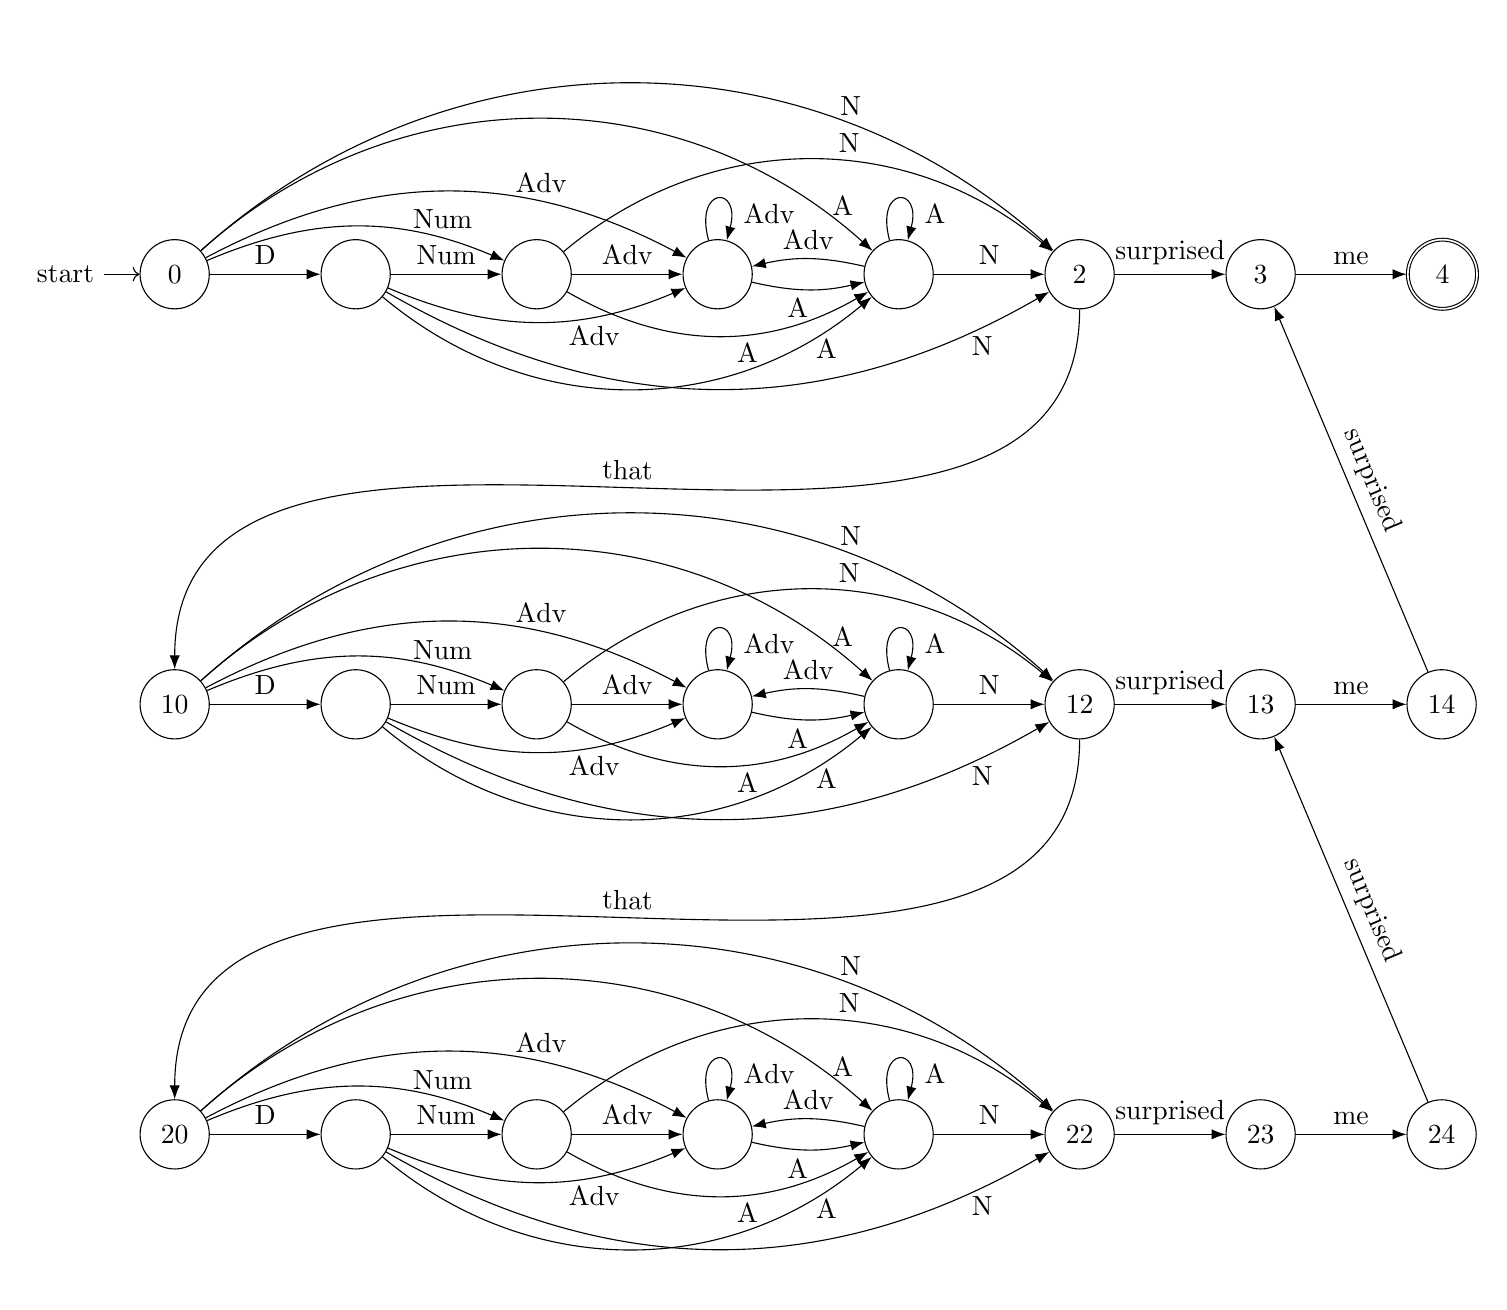
\begin{tikzpicture}
    %%%%%%%%%%%%%
    %  Level 0  %
    %%%%%%%%%%%%%
    \node[state,initial] (n-0-0) at (0,0) {0};
    \foreach \x [remember=\x as \lastx (initially 0)] in {1,2,3,4} 
        \node[state] (n-0-\x) [right=4em of n-0-\lastx] {};
    \node[state] (n-0-5) [right=4em of n-0-4] {2};

    \draw[headarrow] (n-0-0) to node [above] {D}   (n-0-1);
    \draw[headarrow, bend left=23] (n-0-0) to node [above, pos=.8] {Num} (n-0-2);
    \draw[headarrow, bend left=28] (n-0-0) to node [above, pos=.7] {Adv} (n-0-3);
    \draw[headarrow, bend left=42] (n-0-0) to node [above, pos=.95] {A}   (n-0-4);
    \draw[headarrow, bend left=42] (n-0-0) to node [above, pos=.75] {N}   (n-0-5);

    \draw[headarrow] (n-0-1) to node [above] {Num} (n-0-2);
    \draw[headarrow, bend right=23] (n-0-1) to node [below, pos=.7] {Adv} (n-0-3);
    \draw[headarrow, bend right=40] (n-0-1) to node [below, pos=.9] {A}   (n-0-4);
    \draw[headarrow, bend right=30] (n-0-1) to node [below, pos=.9] {N}   (n-0-5);

    \draw[headarrow] (n-0-2) to node [above] {Adv} (n-0-3);
    \draw[headarrow, bend right=30] (n-0-2) to node [below, pos=.6] {A}   (n-0-4);
    \draw[headarrow, bend left=40]  (n-0-2) to node [above, pos=.58] {N}   (n-0-5);

    \draw[headarrow, bend right=13] (n-0-3) to node [below, pos=.4] {A} (n-0-4);
    \draw[headarrow] (n-0-3) to [loop above] node [right, pos=.2] {\quad Adv} (n-0-3);

    \draw[headarrow] (n-0-4) to node [above] {N} (n-0-5);
    \draw[headarrow] (n-0-4) to [loop above] node [right, pos=.2] {\quad A} (n-0-4);
    \draw[headarrow, bend right=13] (n-0-4) to node [above] {Adv} (n-0-3);

    % continue with normal automaton at level 0
    \node[state] (0-3) [right=4em of n-0-5] {3};
    \node[state,accepting] (0-4) [right=4em of 0-3] {4};

    \draw[headarrow] (n-0-5) to node [above] {surprised} (0-3);
    \draw[headarrow] (0-3) to node [above] {me} (0-4);


    %%%%%%%%%%%%%
    %  Level 1  %
    %%%%%%%%%%%%%
    
    \node[state] (n-1-0) [below=13em of n-0-0] {10};
    \foreach \x [remember=\x as \lastx (initially 0)] in {1,2,3,4} 
        \node[state] (n-1-\x) [right=4em of n-1-\lastx] {};
    \node[state] (n-1-5) [right=4em of n-1-4] {12};

    \draw[headarrow] (n-1-0) to node [above] {D}   (n-1-1);
    \draw[headarrow, bend left=23] (n-1-0) to node [above, pos=.8] {Num} (n-1-2);
    \draw[headarrow, bend left=28] (n-1-0) to node [above, pos=.7] {Adv} (n-1-3);
    \draw[headarrow, bend left=42] (n-1-0) to node [above, pos=.95] {A}   (n-1-4);
    \draw[headarrow, bend left=42] (n-1-0) to node [above, pos=.75] {N}   (n-1-5);

    \draw[headarrow] (n-1-1) to node [above] {Num} (n-1-2);
    \draw[headarrow, bend right=23] (n-1-1) to node [below, pos=.7] {Adv} (n-1-3);
    \draw[headarrow, bend right=40] (n-1-1) to node [below, pos=.9] {A}   (n-1-4);
    \draw[headarrow, bend right=30] (n-1-1) to node [below, pos=.9] {N}   (n-1-5);

    \draw[headarrow] (n-1-2) to node [above] {Adv} (n-1-3);
    \draw[headarrow, bend right=30] (n-1-2) to node [below, pos=.6] {A}   (n-1-4);
    \draw[headarrow, bend left=40]  (n-1-2) to node [above, pos=.58] {N}   (n-1-5);

    \draw[headarrow, bend right=13] (n-1-3) to node [below, pos=.4] {A} (n-1-4);
    \draw[headarrow] (n-1-3) to [loop above] node [right, pos=.2] {\quad Adv} (n-1-3);

    \draw[headarrow] (n-1-4) to node [above] {N} (n-1-5);
    \draw[headarrow] (n-1-4) to [loop above] node [right, pos=.2] {\quad A} (n-1-4);
    \draw[headarrow, bend right=13] (n-1-4) to node [above] {Adv} (n-1-3);

    % continue with normal automaton at level 1
    \node[state] (1-3) [right=4em of n-1-5] {13};
    \node[state] (1-4) [right=4em of 1-3] {14};

    \draw[headarrow] (n-1-5) to node [above] {surprised} (1-3);
    \draw[headarrow] (1-3) to node [above] {me} (1-4);

    %%%%%%%%%%%%%
    %  Level 2  %
    %%%%%%%%%%%%%
    
    \node[state] (n-2-0) [below=13em of n-1-0] {20};
    \foreach \x [remember=\x as \lastx (initially 0)] in {1,2,3,4} 
        \node[state] (n-2-\x) [right=4em of n-2-\lastx] {};
    \node[state] (n-2-5) [right=4em of n-2-4] {22};

    \draw[headarrow] (n-2-0) to node [above] {D}   (n-2-1);
    \draw[headarrow, bend left=23] (n-2-0) to node [above, pos=.8] {Num} (n-2-2);
    \draw[headarrow, bend left=28] (n-2-0) to node [above, pos=.7] {Adv} (n-2-3);
    \draw[headarrow, bend left=42] (n-2-0) to node [above, pos=.95] {A}   (n-2-4);
    \draw[headarrow, bend left=42] (n-2-0) to node [above, pos=.75] {N}   (n-2-5);

    \draw[headarrow] (n-2-1) to node [above] {Num} (n-2-2);
    \draw[headarrow, bend right=23] (n-2-1) to node [below, pos=.7] {Adv} (n-2-3);
    \draw[headarrow, bend right=40] (n-2-1) to node [below, pos=.9] {A}   (n-2-4);
    \draw[headarrow, bend right=30] (n-2-1) to node [below, pos=.9] {N}   (n-2-5);

    \draw[headarrow] (n-2-2) to node [above] {Adv} (n-2-3);
    \draw[headarrow, bend right=30] (n-2-2) to node [below, pos=.6] {A}   (n-2-4);
    \draw[headarrow, bend left=40]  (n-2-2) to node [above, pos=.58] {N}   (n-2-5);

    \draw[headarrow, bend right=13] (n-2-3) to node [below, pos=.4] {A} (n-2-4);
    \draw[headarrow] (n-2-3) to [loop above] node [right, pos=.2] {\quad Adv} (n-2-3);

    \draw[headarrow] (n-2-4) to node [above] {N} (n-2-5);
    \draw[headarrow] (n-2-4) to [loop above] node [right, pos=.2] {\quad A} (n-2-4);
    \draw[headarrow, bend right=13] (n-2-4) to node [above] {Adv} (n-2-3);

    % continue with normal automaton at level 2
    \node[state] (2-3) [right=4em of n-2-5] {23};
    \node[state] (2-4) [right=4em of 2-3] {24};

    \draw[headarrow] (n-2-5) to node [above] {surprised} (2-3);
    \draw[headarrow] (2-3) to node [above] {me} (2-4);

    %%%%%%%%%%%%%%%%%%%%%%
    %  Connecting edges  %
    %%%%%%%%%%%%%%%%%%%%%%
    
    \draw[headarrow] (n-0-5) to [out=270, in=90] node [above,sloped] {that} (n-1-0);
    \draw[headarrow] (n-1-5) to [out=270, in=90] node [above,sloped] {that} (n-2-0);
    \draw[headarrow] (1-4) to node [above,sloped] {surprised} (0-3);
    \draw[headarrow] (2-4) to node [above,sloped] {surprised} (1-3);
\end{tikzpicture}
\end{document}
